\documentclass[a4paper]{report}
%\documentclass[a4paper,twoside,openright]{report}
\usepackage[utf8]{inputenc}
\usepackage[T1]{fontenc}
\usepackage[ngerman,english]{babel}
\usepackage{titlesec}
\usepackage{subfigure}
\usepackage{graphicx}
\usepackage{parskip}
\usepackage{lmodern}
\usepackage{adjustbox}
\usepackage{tikz}
\usepackage{amsmath}
\usepackage{amssymb}
\usepackage{caption}

\usepackage{multirow}
\usepackage{listings}
\usepackage{algorithm}
\usepackage{algpseudocode}
\usepackage{pgfplots}
\usepackage{pdflscape}
\usepackage[hidelinks]{hyperref}
\usetikzlibrary{arrows,shapes,fit,positioning}
\usetikzlibrary{decorations.pathmorphing}
\usetikzlibrary{decorations.markings}

\pgfplotsset{compat=1.18}

\titleformat{\chapter}[display]
{\normalfont\huge\bfseries}{\chaptertitlename\ \thechapter}{20pt}{\Huge}

% configure autoref
\addto\extrasenglish{
	\def\chapterautorefname{Chapter}
	\def\subsectionautorefname{Subsection}
	\def\sectionautorefname{Section}
}

% this alters "before" spacing (the second length argument) to 0
\titlespacing*{\chapter}{0pt}{-50pt}{20pt}

\author{}
\date{\today}
\begin{document}
\pagestyle{empty}
\begin{titlepage}
\begin{center}
  % Upper part of the page  
	
\includegraphics[width=10cm,clip,trim=0 0 0 0\textwidth]{rptu}\\[2cm]
	% {
	% 	\linespread{1.5}\selectfont
	% 	\textsc{\LARGE Rheinland-Pfälzische Technische Universität Kaiserslautern-Landau}\\[0.5cm]
	% }
  \textsc{\large Fachbereich Informatik}\\[1.5cm]
	\vfill
  \textsc{\Large Master's Thesis}\\[0.5cm]
{
  \linespread{1.0}\selectfont
{\LARGE   \textsc{Creating and Benchmarking Learned Database Components using LLMs}\\[2cm]}
}

  { \Large
  Author:\\
	Preksha Rajesh Shah\\[2cm]
  {\small submitted on: \\
  \today}
  }\\[1cm]

  Supervisor\\
  Angjela Davitkova\\[1cm]
  Reviewers\\
  Prof. Dr.-Ing. Sebastian Michel\\

  
\end{center}
\end{titlepage}

%
\cleardoublepage


\begin{abstract}
Lorem ipsum
\end{abstract}

\cleardoublepage

\selectlanguage{ngerman}
\begin{abstract}
Lorem ipsum
\end{abstract}
\selectlanguage{english}

\tableofcontents
\thispagestyle{empty}
\listoffigures
\thispagestyle{empty}
\begingroup
\thispagestyle{empty}
\let\clearpage\relax
\vspace{3cm}
\listofalgorithms
\let\clearpage\relax
\vspace{3cm}
\listoftables
\endgroup
\thispagestyle{empty}


%%% 
%%% Add your inputs here
%%%

% !TEX root =  main.tex

\chapter{Introduction}
\label{chap:introduction}
\pagestyle{plain}
\setcounter{page}{1}

\section{Problem Statement}

Query optimization in relational databases hinges on cardinality estimation---predicting how many rows a query will return before actually executing it. Get the estimate right and the optimizer picks a fast execution plan. Get it wrong and the plan can be orders of magnitude slower than necessary. Traditional estimators lean on assumptions like attribute independence and uniform value distributions that rarely hold in practice, and the resulting errors compound across joins, leading to plans that are far from optimal.

Over the past few years, learned cardinality estimators have shown that neural networks can do a better job. The Multi-Set Convolutional Network (MSCN) by Kipf et al.~\cite{DBLP:conf/cidr/KipfKRLBK19} demonstrated that a relatively simple deep learning model can capture cross-table correlations that rule-based estimators miss entirely. But learned models come with their own cost: they need large quantities of labeled training data, and each label requires executing a query on a live database to record its true row count. On a complex schema this execution-based labeling can take hours, making it the dominant bottleneck in any pipeline that trains learned estimators from scratch.

Meanwhile, large language models have become remarkably good at generating SQL. Work like SQLStorm~\cite{DBLP:journals/pvldb/SchmidtLBN25} has shown that LLMs can produce diverse, realistic query workloads at scale when given a schema and a well-crafted prompt. But generating queries is only half the problem. Those queries still need to be executed to obtain labels, and that execution cost remains.

The question this thesis addresses is: can we close the loop---generate a large, diverse pool of queries with an LLM, then use active learning to pick only the most informative ones for labeling---so that we get a good estimator without paying the full cost of executing every query in the pool?

\section{Proposed Approach}

We treat the LLM not as a runtime component but as a data factory. Given a database schema, the LLM generates thousands of synthetic \texttt{SELECT COUNT(*)} queries. These queries are validated, filtered, and encoded into the tensor format that MSCN expects. Then, instead of labeling them all, we use active learning to identify the queries that the model is most uncertain about and label only those. The model trains on the labeled subset, its uncertainty shifts, and the next round of selection targets different queries. After several rounds the model has seen a compact but highly informative training set.

The whole process is packaged as an automated, schema-agnostic pipeline. A researcher points it at a database, specifies a few hyperparameters, and walks away. The pipeline generates queries, validates them through four filtering layers, labels the selected subset, trains the MSCN model, and outputs a full evaluation dashboard. No manual query writing, no template engineering, no human in the loop.

The motivation draws on two bodies of prior work. Wang et al.~\cite{DBLP:journals/pvldb/WangQWWZ21} showed that the diversity and structural properties of the training workload have a profound effect on learned estimator quality, and Davitkova and Michel~\cite{DBLP:journals/corr/abs-2512-20271} demonstrated that generative AI can automate the creation of training data for database components. We build on both: using LLMs for diverse workload generation and active learning for efficient labeling.

\section{Contributions}

This thesis makes four contributions. First, it demonstrates that LLMs can serve as effective workload generators for learned cardinality estimation, producing queries with structural diversity that rivals or exceeds what template-based methods achieve. Second, it integrates active learning into the training loop, showing that uncertainty-based query selection reduces the labeling budget needed to reach a given accuracy level. Third, it packages everything into a fully automated pipeline that works out of the box on any schema with defined foreign keys, lowering the barrier to entry for researchers who want to experiment with learned estimators. Fourth, it provides an extensive experimental evaluation on the IMDB benchmark that quantifies the trade-offs between different acquisition strategies, workload sizes, and training configurations.
% !TEX root =  main.tex
\chapter{Background}
\label{chap:background}
\pagestyle{plain}

\section{Learned Database Systems and Cardinality Estimation}

Modern database systems use query optimizers to optimize queries for efficient execution. At the heart of query optimization is cardinality estimation. Cardinality estimation is used to predict the number of tuples that are generated during intermediate steps of query execution. The estimates are used to optimize queries and improve performance. However, small errors in cardinality estimation can lead to poor query optimization and performance. Conventional cardinality estimation techniques use statistical estimates such as histograms and sampling. Other techniques include making assumptions such as attribute independence and uniform distribution of values. Although conventional techniques are computationally efficient, they do not reflect real-world data characteristics. Real-world data has complex correlations among attributes and tables, especially for join-heavy queries. As such, conventional techniques often yield poor estimates for queries with multiple predicates and joins.

In addition to inaccuracies caused by independence assumptions, another limitation of traditional approaches lies in their inability to adapt dynamically to evolving data distributions. In real-world applications, data is continuously updated, and query workloads may change over time. Static statistical summaries often fail to capture these changes effectively, leading to outdated estimates and suboptimal execution plans. This problem becomes more severe in large-scale systems where maintaining accurate statistics is itself a costly operation. As a result, there has been a growing interest in approaches that can learn directly from data and adapt to changing workloads.

This limitation has motivated the exploration of learned database systems, where machine learning models replace traditional components. Instead of relying on predefined assumptions, these models learn patterns directly from data, enabling them to capture correlations that are otherwise difficult to model. Learned cardinality estimation is one of the most actively studied areas within this paradigm. These models aim to generalize across different query structures and data distributions, providing more robust and accurate estimates compared to traditional techniques.

\section{MSCN and Deep Learning-based Estimation}

One important advancement in the area of learning-based query cardinality estimation is the development of a new technique called Multi-Set Convolutional Network (MSCN), proposed by Kipf et al. in\cite{DBLP:conf/cidr/KipfKRLBK19}. The technique reformulates query cardinality estimation as a supervised learning task, where query result sizes are estimated based on query structures.

The basic idea behind the MSCN technique is that it represents queries in the form of sets. Unlike traditional methods, where a query is simply represented as a string of characters, MSCN represents a query as three different sets, namely tables, joins, and predicates. Each set is processed separately using shared layers of a neural network. The basic idea behind this is to make the query invariant to the ordering of query components, which is important because the semantics of a query do not depend on the order in which tables and predicates are listed.

The other key feature of the MSCN is its use of bitmap-based sampling. In the process, a subset of the tuples in a given base table is sampled, and the predicates are applied to the sample to produce bitmaps. The bitmaps then represent the query predicates that are satisfied, and this additional information helps the model to better account for the correlations between the predicates and the data.

In addition, the MSCN uses normalization to ensure that the cardinality estimates are within a certain range that can be learned by the model. This is crucial, especially considering that the cardinality estimates can differ considerably across queries.The MSCN uses loss functions that involve relative errors, as opposed to absolute errors, which is more appropriate for query optimization tasks.

Despite its strong performance, MSCN depends heavily on labeled training data. Each training example requires a query and its true cardinality, which is obtained by executing the query on a database. As query complexity increases, the cost of execution grows significantly, making it difficult to scale the training process. This limitation highlights a fundamental challenge in learned database systems: the high cost of data generation. In addition, the reliance on execution makes it difficult to quickly generate new training data when schemas or workloads change.

\section{Workload Sensitivity and Challenges}

The performance of learned cardinality estimators not only depends on the architecture used but also on the nature and characteristics of the training workload. The study conducted by Wang et al. \cite{DBLP:journals/pvldb/WangQWWZ21} offers a comprehensive analysis on how different query properties influence the performance of learned cardinality estimators.

For example, a learned model may not perform well when it is tested on queries that have different types of predicates, such as range predicates, when it is only trained on queries that have equality predicates. Similarly, a query may have high selectivity and join complexity, causing a large estimation error. This example again emphasizes that the training data should be highly diverse.

Another important aspect to be considered is related to workload shift, where the query distribution is different from the training distribution. In this case, learned models may not perform well, and this again emphasizes that the training data should be highly diverse. Moreover, the interaction between multiple query features, such as the number of joins and predicate selectivity, can further complicate the estimation process. These interactions are often difficult to model explicitly, which reinforces the importance of exposing models to a wide variety of query patterns during training.

\section{LLM-based SQL Generation}

Recently, large language models have been recognized as effective means for generating structured data. In this regard, the SQLStorm framework\cite{DBLP:journals/pvldb/SchmidtLBN25} has been presented to show that LLMs can be effectively used to produce large volumes of varied and realistic SQL queries. In this regard, the SQLStorm framework exploits the capabilities of schema-informed prompting to produce varied and realistic queries.

Unlike other query generation techniques that are based on template-based and rule-based approaches, LLMs can be effectively used to produce queries that can capture a wide range of query patterns. This is one of the main reasons that LLMs can be effectively used to produce training datasets for learning-based query generation techniques. In addition to this, LLMs can be effectively used to produce queries that are not included in existing workloads. This allows for the exploration of new query patterns.

Another important advantage of LLM-based generation is its ability to incorporate semantic understanding of schemas. By conditioning on table and column descriptions, LLMs can generate queries that are not only syntactically correct but also semantically meaningful. This capability is particularly useful when dealing with complex schemas, where manual query generation becomes challenging.

Although LLMs can be effectively used to produce queries, they do not have the capability to produce the labels that are associated with the queries. This means that the produced queries have to be executed to produce labels. This is one of the main drawbacks of using LLMs for query generation, as it reintroduces the dependency on database execution.

\section{Generative AI for Database Components}

The base paper \cite{DBLP:journals/corr/abs-2512-20271} attempts to address this data generation bottleneck through a framework that utilizes generative models to automatically generate training data for learned database components. The basic idea is to utilize LLMs to automatically generate realistic SQL queries, thereby reducing reliance on manually collected query logs.
This is a major departure from the traditional way learned database systems have been designed. By automating query generation, it is possible to generate large and varied datasets to support a wide range of query types. The framework also outlines how generative models can be incorporated into the learning pipeline to support data generation.

An important contribution of this work is the structured pipeline it proposes, where query generation, validation, execution, and model training are integrated into a unified framework. This pipeline ensures that generated queries are not only diverse but also executable and meaningful within the given schema. The use of prompt engineering and iterative refinement further improves the quality of generated queries.

One limitation of this framework is that it relies on executing the generated queries to obtain ground truth labels. While query generation is now automated, label generation is computationally intensive and thus limits scalability. This is where a completely synthetic method is proposed, where query and label generation can be performed without relying on database execution. This shift represents a natural evolution of the framework, aiming to remove the remaining bottleneck in the data generation process.

\section{Active Learning for Data Efficiency}

Active learning helps in developing a framework for improving data efficiency, which can be done through the selection of the best data samples for learning. As discussed in \cite{DBLP:journals/tnn/LiWCJDO25}, not all data samples are equally important in improving the performance of the model. This way, it is possible to attain high accuracy with less data.

In the context of LQE using learned cardinality estimation, active learning helps in improving the efficiency of the process of query labeling. Instead of labeling all the generated queries, the model can be improved through the selection of the best queries in improving the performance of the model. This selection of the best queries can be done using the uncertainty of the model.

In addition to uncertainty-based selection, active learning can also incorporate diversity-based sampling, where queries that represent different regions of the query space are selected. This ensures that the model is exposed to a wide range of patterns while avoiding redundancy in the training data. Such strategies are particularly useful when working with large volumes of synthetically generated data.

The integration of active learning with the process of synthetic data generation helps in improving the efficiency of the learning process. LLMs are capable of generating a wide variety of data samples in the form of queries. Active learning helps in the selection of the best data samples, thus improving the efficiency of the learning process.

\section{Data Diversity, Personas, and KL Divergence}

Diversity in the generated data is a critical factor to be taken into consideration for the training of strong models. The PAARS\cite{DBLP:journals/corr/abs-2503-24228} framework proposes the use of personas for generating diverse and realistic data. Personas help in the simulation of diverse behavior, which enables the generation of diverse data.

In order to test the quality of the generated data, the PAARS framework uses the KL divergence as a similarity metric between the generated data and real-world data. The KL divergence is a measure of the dissimilarity between two probability distributions, which can be used to test the similarity between the generated data and real-world data, especially in the case of SQL queries.

In the context of query generation, KL divergence can be applied to distributions over query features such as the number of joins, predicate types, and selectivity ranges. By comparing these distributions between synthetic and real workloads, it is possible to evaluate whether the generated data accurately reflects real-world patterns. This provides a quantitative basis for improving the quality of synthetic datasets.

\section{Local Model Hosting for Reproducibility}

The practical deployment of LLMs for data generation requires careful consideration of reproducibility, privacy, and cost. In this work, we adopt a local hosting strategy using the Ollama framework, which enables running open-source language models entirely on the researcher's own hardware. This choice offers several important benefits for scientific experimentation. Local hosting eliminates dependency on external API services, ensuring that experiments are not affected by changes in third-party model versions, pricing, or availability. It also preserves data privacy, as database schemas and query workloads never leave the local environment. Furthermore, local inference provides consistent latency characteristics and enables full control over model parameters such as temperature and token limits, supporting reproducible experimental conditions.

\section{Summary and Motivation}

The background provided in this section points to the evolution of learned database systems, starting with conventional estimators, followed by machine learning models, and then moving on to the latest generative models. While the MSCN \cite{DBLP:conf/cidr/KipfKRLBK19} paper proves the efficiency of learned models, it also points to the disadvantage of data generation. Subsequent papers focus on the need for diversity in the workload\cite{DBLP:journals/pvldb/WangQWWZ21} and the application of LLMs in query generation \cite{DBLP:journals/pvldb/SchmidtLBN25}.

However, the conventional methods are all based on execution-based labeling, which is not scalable. This thesis, with the help of insights provided by generative models, active learning \cite{DBLP:journals/tnn/LiWCJDO25}, and diversity-aware models, proposes the application of LLMs in generating both the query and the label, thus using the learned model as the final database component.
\input{relatedwork}
% !TEX root =  main.tex
\chapter{Approach}
\label{chap:approach}
\pagestyle{plain}

Training a learned cardinality estimator well requires two things that are at odds with each other: a large, diverse set of labeled queries and a limited budget for obtaining those labels. Each label demands executing a query on a live database, which is slow and expensive. This chapter lays out our strategy for resolving that tension. We walk through the pipeline that ties query generation, labeling, feature extraction, active learning, and evaluation into one continuous workflow, and then explain what makes this framework practical for real research.


\section{System Architecture}

The system chains six stages together into a single automated run. Figure~\ref{fig:system_overview} shows how data flows from the raw database schema all the way to a trained estimator and its evaluation dashboard.

\begin{figure}[htbp]
\centering
\resizebox{\textwidth}{!}{%
\begin{tikzpicture}[
    node distance=1.6cm and 1.8cm,
    block/.style={draw, rectangle, rounded corners=4pt, minimum width=3cm, minimum height=1.1cm, align=center, font=\small},
    arrow/.style={->, thick, >=stealth}
]
    % Row 1: Data Generation
    \node [block, fill=blue!25] (schema) {Database Schema\\+ Statistics};
    \node [block, fill=blue!25, right=of schema] (llm) {LLM Query\\Generation};
    \node [block, fill=green!25, right=of llm] (validation) {Multi-Layer\\SQL Validation};

    % Row 2: Data Processing
    \node [block, fill=yellow!25, below=of schema] (format) {MSCN Format\\Conversion};
    \node [block, fill=orange!25, below=of llm] (labeling) {Database\\Labeling};
    \node [block, fill=red!25, below=of validation] (bitmap) {Bitmap\\Generation};

    % Row 3: Learning
    \node [block, fill=purple!25, below=of format] (al) {Active Learning\\Acquisition};
    \node [block, fill=purple!25, below=of labeling] (training) {MSCN Model\\Training};
    \node [block, fill=cyan!25, below=of bitmap] (evaluation) {Evaluation \&\\Visualization};

    % Arrows Row 1
    \draw [arrow] (schema) -- (llm);
    \draw [arrow] (llm) -- (validation);

    % Arrows Row 1 to Row 2
    \draw [arrow] (validation) -- (format);
    \draw [arrow] (format) -- (labeling);
    \draw [arrow] (labeling) -- (bitmap);

    % Arrows Row 2 to Row 3
    \draw [arrow] (bitmap) -- (al);
    \draw [arrow] (al) -- (training);
    \draw [arrow] (training) -- (evaluation);

    % Feedback loop
    \draw [arrow, dashed, red!60] (evaluation.south) -- ++(0,-0.6) -| (al.south) node[pos=0.25, below, font=\scriptsize, text=gray] {Feedback Loop};

    % Stage labels
    \node [above=0.3cm of llm, font=\footnotesize\bfseries, text=blue!70] {Stage 1: Generation};
    \node [left=0.6cm of format, font=\footnotesize\bfseries, text=orange!70, align=right] {Stage 2:\\Processing};
    \node [below=0.3cm of training, font=\footnotesize\bfseries, text=purple!70] {Stage 3: Learning};

\end{tikzpicture}%
}
\caption{End-to-end pipeline from schema ingestion through query generation, validation, labeling, and active learning to final model evaluation. The dashed feedback loop represents the iterative active learning cycle.}
\label{fig:system_overview}
\end{figure}


\section{Pipeline Walkthrough}

Everything starts with query generation. The pipeline feeds the database schema and column statistics to a large language model and asks it to produce batches of \texttt{SELECT COUNT(*)} queries. Because LLMs have absorbed millions of SQL examples during pre-training, the queries they produce tend to look like something a real analyst might write---varied join structures, plausible predicate values, a mix of simple and complex patterns. A deterministic synthetic generator is also available for situations where an LLM is impractical. Chapter~\ref{chap:query_generation} covers the prompt design, diversity mechanisms, and the four-layer validation filter that weeds out malformed or unsupported queries before they enter the pipeline.

Validated queries then need ground truth labels. For each query, the pipeline reconstructs a \texttt{SELECT COUNT(*)} statement, executes it against PostgreSQL, and records the row count. This labeling step is by far the most expensive part of the process: a single complex join can take seconds, and labeling thousands of queries can take hours. It is exactly this cost that makes active learning worthwhile. Instead of labeling every query up front, the pipeline labels only a carefully chosen subset and defers the rest.

Before queries reach the neural network they are converted into fixed-size tensors. Each query is decomposed into three sets---tables, predicates, and joins---and each element is encoded as a combination of one-hot vectors and, for tables, a bitmap that indicates which pre-sampled rows satisfy the query's filters. These bitmaps give the model a window into the actual data distribution, not just the query structure. The complete encoding process and MSCN architecture are described in Chapter~\ref{chap:training_approach}.

The active learning loop ties everything together. It begins by randomly labeling a small seed set, trains the MSCN model on that seed, then asks: which of the remaining unlabeled queries would teach the model the most? The acquisition function scores every candidate, the top-scoring queries are labeled and added to the training set, and the model is retrained. This cycle repeats for several rounds. Each round the model gets a little better, and each round it gets better at deciding what to learn next. Three acquisition strategies are supported---random, uncertainty-based, and Monte Carlo dropout---each representing a different trade-off between computation and sample efficiency. Chapter~\ref{chap:active_learning} presents the active learning framework in detail.

The final stage produces a dashboard of diagnostic plots: learning curves showing how accuracy improves with each round, scatter plots of predicted versus actual cardinalities, Q-error distributions, and workload diversity profiles. These visualizations make it straightforward to judge both the quality of the generated data and the performance of the trained estimator. Experimental results are presented in Chapter~\ref{chap:experiments}.


\section{Why This Framework}

Several properties set this framework apart from earlier efforts at learned cardinality estimation.

The pipeline is schema-agnostic. Hand it a set of table definitions, column types, and foreign key relationships and it will generate queries, validate them, extract features, and train a model without a single line of manual configuration. Swap the IMDB schema for a retail database and the same code runs unchanged. That kind of portability matters because learned estimators are only useful if they can be retrained cheaply when the schema or the data evolves.

Every stage of the pipeline is designed as a replaceable module. The query generator currently calls a locally hosted Llama model through Ollama, but swapping it for GPT-4 or a template-based generator requires changing one configuration flag, not rewriting the pipeline. The same is true of the acquisition strategy used during active learning and the neural network architecture used for estimation. Researchers can therefore isolate the effect of any single component without confounding variables from the rest of the system.

Robustness is built in rather than bolted on. Queries that time out are retried with back-off; queries that fail permanently receive a safe fallback label and the pipeline moves on. Thousands of queries can be processed overnight without a human watching the terminal.

Finally, every experiment is fully reproducible. Random seeds propagate through Python, NumPy, and PyTorch. All hyperparameters are logged to disk alongside the results, and timestamped output directories prevent one run from accidentally overwriting another.
% !TEX root =  main.tex
\chapter{Query Generation Approach}
\label{chap:query_generation}
\pagestyle{plain}

This chapter presents the detailed approach for generating diverse, realistic SQL query workloads using large language models. Query generation is the foundational stage of the pipeline, as the quality and diversity of generated queries directly impacts the effectiveness of downstream model training. We describe the prompt engineering strategy, the multi-layer validation pipeline, the format conversion process, and the synthetic fallback generator.


\section{LLM-Based Query Generation}

Traditional approaches to generating training workloads for learned database components fall into two broad categories: manual collection from query logs and synthetic generation using template-based or random sampling methods. Query logs require access to production systems, raise privacy concerns, and may not cover the full spectrum of query patterns needed for robust model training. Template-based generators, on the other hand, produce queries that are syntactically valid but often lack the structural variety and realistic predicate distributions found in real workloads. Random sampling can generate uniformly distributed queries but misses the complex correlations and patterns that characterize real-world usage.

Large language models offer a compelling alternative because they have been trained on vast corpora of natural language and code, including millions of SQL queries. This training enables them to generate queries that exhibit realistic structural patterns, meaningful predicate combinations, and diverse join topologies without explicit programming of these patterns. Our framework uses the Ollama platform to host and serve LLMs locally, ensuring data privacy and eliminating dependency on external API services. The default model is Llama~3.2, selected for its strong code generation capabilities and reasonable computational requirements. The system interacts with Ollama through its REST API, enabling seamless switching between different model sizes and families without code changes.


\section{Prompt Design}

The quality of LLM-generated queries critically depends on the prompt design. We employ a carefully structured prompt template that provides the model with sufficient context to generate valid, diverse queries while constraining output to the supported query fragment. The prompt consists of five hierarchically organized components, as illustrated in Figure~\ref{fig:prompt_structure}: a role assignment that establishes the LLM as a SQL workload generator, the complete database schema context including DDL statements with table names, columns, data types, and foreign key relationships, optional column statistics providing min/max values for numeric columns to enable realistic predicate generation, a set of strict generation rules, and an output format specification.

\begin{figure}[htbp]
\centering
\begin{tikzpicture}[
    block/.style={draw, rectangle, rounded corners=3pt, minimum width=13cm, minimum height=1.3cm, text centered, font=\small},
    arrow/.style={->, thick, >=stealth},
    node distance=1.5cm
]
    \node [block, fill=blue!15] (role) {\textbf{1. Role Assignment}: ``You are a SQL query workload generator for a database.''};
    \node [block, fill=green!15, below=of role] (schema) {\textbf{2. Schema Context}: Complete DDL with table names, columns, types, and relationships};
    \node [block, fill=yellow!15, below=of schema] (stats) {\textbf{3. Column Statistics}: Min/max values and cardinalities for numeric columns};
    \node [block, fill=orange!15, below=of stats] (rules) {\textbf{4. Generation Rules}: Strict constraints on query structure and complexity};
    \node [block, fill=red!15, below=of rules] (output) {\textbf{5. Output Format}: JSON array specification with example queries};

    \draw [arrow] (role) -- (schema);
    \draw [arrow] (schema) -- (stats);
    \draw [arrow] (stats) -- (rules);
    \draw [arrow] (rules) -- (output);

    \node [left=0.3cm of role, font=\scriptsize, text=gray, rotate=90, anchor=south] {Context};
    \node [left=0.3cm of rules, font=\scriptsize, text=gray, rotate=90, anchor=south] {Constraints};

\end{tikzpicture}
\caption{Structure of the LLM prompt template, consisting of five hierarchically organized components that guide the model from context understanding to constrained output generation.}
\label{fig:prompt_structure}
\end{figure}

The generation rules are critical for ensuring that the produced queries are compatible with the MSCN encoding. The prompt enforces that all queries use the \texttt{SELECT COUNT(*)} format exclusively, involve one to three tables from the provided schema with proper aliases, include join conditions using defined foreign key relationships, and use only simple comparison operators (\texttt{=}, \texttt{<}, \texttt{>}) with numeric values connected by \texttt{AND}. Constructs such as \texttt{OR}, \texttt{IN}, \texttt{LIKE}, \texttt{BETWEEN}, subqueries, and aggregations are explicitly forbidden. These constraints are necessary because the MSCN encoding assumes a specific query structure where predicates are AND-connected simple comparisons over numeric columns; queries violating these constraints would either fail during encoding or produce incorrect feature representations.

The prompt instructs the LLM to return queries as a JSON array of objects, each containing a single \texttt{"sql"} field. This structured output format enables reliable parsing and reduces the need for complex text extraction. A fallback regex-based extraction is used when the LLM includes additional text around the JSON.


\section{Diversity and Batch Generation}

To maximize workload diversity across generation batches, we employ a rotating set of diversity hints. Each batch receives a different textual hint that steers the LLM toward generating queries with specific characteristics, ranging from single-table queries with various filters to complex three-table joins with multiple predicates, and from point lookups to queries with extreme selectivities. The hint index is computed as $(\lfloor \text{existing\_count} / \text{batch\_size} \rfloor) \bmod 5$, ensuring systematic rotation through all diversity profiles as generation progresses. This approach avoids the mode collapse problem where the LLM repeatedly generates structurally similar queries.

Generating all queries in a single LLM call would exceed token limits and reduce diversity. Instead, the system generates queries in configurable batches, with the total number of batches determined by $\lceil \text{total\_queries} / \text{batch\_size} \rceil$. Each batch receives a fresh prompt with the current diversity hint, ensuring variety across the full workload. LLM generation is inherently stochastic and may fail due to network errors, malformed JSON output, or hallucination. Each batch is therefore retried up to three times with increasing delays between attempts, achieving near-complete batch success rates in practice. Algorithm~\ref{alg:batch_generation} presents the batch generation procedure.

\begin{algorithm}[htbp]
\caption{LLM-Based Query Generation}
\label{alg:batch_generation}
\begin{algorithmic}[1]
\State Determine how many batches are needed to reach the target number of queries
\For{each batch}
    \State Choose a diversity hint based on how many queries have been generated so far
    \State Construct a prompt containing the database schema, column statistics, and the chosen hint
    \For{up to 3 attempts}
        \State Send the prompt to the language model and receive a response
        \State Try to extract valid SQL queries from the response
        \If{at least one valid query was found}
            \State Add the extracted queries to the collection and move to the next batch
        \EndIf
    \EndFor
\EndFor
\State \Return the collected queries, trimmed to the target count
\end{algorithmic}
\end{algorithm}


\section{Multi-Layer Validation Pipeline}

Raw LLM output must undergo rigorous validation before entering the training pipeline. Despite careful prompt engineering, LLMs can produce queries that are syntactically invalid, reference non-existent schema elements, or use unsupported SQL constructs. Our validation pipeline applies four sequential filtering stages, each progressively more expensive but more thorough, as illustrated in Figure~\ref{fig:validation_pipeline}.

\begin{figure}[htbp]
\centering
\begin{tikzpicture}[
    node distance=1.8cm,
    block/.style={draw, rectangle, rounded corners=3pt, minimum width=5.5cm, minimum height=1.1cm, align=center, font=\small},
    reject/.style={draw, rectangle, rounded corners=3pt, minimum width=2.5cm, minimum height=0.8cm, align=center, font=\small, fill=red!15},
    arrow/.style={->, thick, >=stealth},
    rarrow/.style={->, thick, >=stealth, red!70},
]
    \node [block, fill=gray!15] (raw) {Raw LLM Output (N queries)};
    \node [block, fill=blue!15, below=of raw] (struct) {Layer 1: Structural Validation\\{\scriptsize Regex-based keyword filtering}};
    \node [block, fill=green!15, below=of struct] (parse) {Layer 2: SQL Parsing\\{\scriptsize FROM/WHERE clause extraction}};
    \node [block, fill=yellow!15, below=of parse] (schema) {Layer 3: Schema Validation\\{\scriptsize Table/column existence checks}};
    \node [block, fill=orange!15, below=of schema] (format) {Layer 4: Format Conversion\\{\scriptsize MSCN-compatible structure}};
    \node [block, fill=green!30, below=of format] (valid) {Valid Queries ($\leq$ N)};

    \draw [arrow] (raw) -- (struct);
    \draw [arrow] (struct) -- (parse);
    \draw [arrow] (parse) -- (schema);
    \draw [arrow] (schema) -- (format);
    \draw [arrow] (format) -- (valid);

    \node [reject, right=2.5cm of struct] (r1) {Reject: Forbidden\\keywords found};
    \node [reject, right=2.5cm of parse] (r2) {Reject: Parse\\failure};
    \node [reject, right=2.5cm of schema] (r3) {Reject: Unknown\\table/column};
    \node [reject, right=2.5cm of format] (r4) {Reject: Conversion\\failure};

    \draw [rarrow] (struct.east) -- (r1.west);
    \draw [rarrow] (parse.east) -- (r2.west);
    \draw [rarrow] (schema.east) -- (r3.west);
    \draw [rarrow] (format.east) -- (r4.west);

\end{tikzpicture}
\caption{Multi-layer validation pipeline for LLM-generated queries. Each layer progressively filters invalid queries, with rejected queries logged for analysis.}
\label{fig:validation_pipeline}
\end{figure}

The first layer is a fast, regex-based filter that rejects queries containing forbidden SQL patterns such as \texttt{OR}, \texttt{IN}, \texttt{LIKE}, \texttt{BETWEEN}, subqueries, and aggregations. This layer catches the most common LLM errors at minimal computational cost. The second layer parses each surviving query to extract its FROM and WHERE clauses, handling both comma-separated join syntax and explicit \texttt{JOIN...ON} syntax and producing a normalized representation of tables, join conditions, and filter predicates.

The third layer validates the parsed query against the database schema, verifying that all referenced table names, column names, and aliases actually exist. Join conditions are checked to confirm that they reference columns participating in defined foreign key relationships. The fourth and final layer converts valid queries from their parsed representation into the MSCN-compatible structured format, decomposing each query into three sets: tables (with aliases), joins (as equality conditions), and predicates (as column-operator-value tuples). This conversion includes operator standardization, value normalization, case normalization, and alias resolution to ensure consistent encoding downstream.


\section{Synthetic Query Generator}

For testing and environments where an LLM is unavailable, the framework includes a deterministic synthetic query generator. This generator produces structurally valid queries using parameterized random sampling based on hardcoded table definitions from the target schema. It uses weighted random selection for table count, biasing toward two-table queries to match typical workload distributions, and all multi-table queries include the central fact table to reflect the star-schema topology of the benchmark database.

Table~\ref{tab:gen_comparison} compares the characteristics of queries produced by the two generation approaches.

\begin{table}[htbp]
\centering
\caption{Comparison of LLM-based and synthetic query generation approaches.}
\label{tab:gen_comparison}
\begin{tabular}{|l|c|c|}
\hline
\textbf{Property} & \textbf{LLM-Based} & \textbf{Synthetic} \\
\hline
Schema adaptability & Automatic & Requires manual updates \\
Predicate diversity & High (learned patterns) & Medium (uniform random) \\
Join topology variety & High & Limited to star schema \\
Value distribution & Realistic (stat-aware) & Uniform within range \\
Validation pass rate & $\sim$95\% & 100\% (by construction) \\
Reproducibility & Non-deterministic & Fully deterministic \\
\hline
\end{tabular}
\end{table}

The LLM-based generator produces higher-quality workloads with greater diversity, while the synthetic generator provides a deterministic, zero-dependency fallback. In practice, the LLM-based generator is recommended for final experiments, while the synthetic generator serves well for rapid development and testing.


\section{Summary}

This chapter presented the detailed approach for generating SQL query workloads using large language models. The key contributions include a structured prompt engineering strategy that achieves high validation pass rates, a four-layer validation pipeline that ensures only well-formed and schema-compatible queries enter the training pipeline, a diversity hint rotation mechanism that prevents mode collapse in generated workloads, and a deterministic synthetic generator for testing environments. The next chapter describes how these generated queries are labeled, encoded, and used to train the MSCN cardinality estimator through active learning.

% !TEX root =  main.tex
\chapter{Training Approach}
\label{chap:training_approach}
\pagestyle{plain}

Getting from a pile of validated SQL queries to a neural network that estimates cardinalities accurately involves several non-trivial steps: labeling each query with its true row count, encoding the query into a fixed-size tensor the network can digest, and training the network with an appropriate loss function. This chapter covers each of these steps. The active learning framework that decides which queries are worth labeling is presented separately in Chapter~\ref{chap:active_learning}.


\section{Database Labeling}

Every supervised model needs labels. In our setting a label is the true cardinality of a query the number of rows it returns. Obtaining that number means actually running the query: reconstructing a \texttt{SELECT COUNT(*)} statement from the query's tables, joins, and predicates, submitting it to PostgreSQL, and recording the result.

This sounds straightforward, but at scale it is the dominant bottleneck of the entire pipeline. A single three-table join over tens of millions of rows can take seconds. Multiply that by a few thousand queries and the labeling stage alone can consume hours of compute. Some queries never finish at all: they hit pathological join orderings or blow up intermediate result sizes, making them impractical to execute within any reasonable time budget.

The pipeline handles these cases pragmatically. Each query runs under a timeout. If it does not finish, it is retried once with a longer deadline. If it still fails, it receives a fallback cardinality of one, the smallest value that keeps the log-scale normalization well-defined. This fallback introduces a small amount of noise into the training data, but in practice the fraction of queries that reach it is low enough that the model's overall accuracy is not materially affected.

The expense of labeling is the single strongest argument for active learning. If every label costs real compute, then choosing which queries to label is not just a nice optimization it is the difference between a pipeline that finishes overnight and one that runs for days.


\section{Feature Extraction and Bitmap Generation}

The MSCN architecture expects three fixed-size tensors as input one for tables, one for predicates, one for joins but real queries have variable numbers of each. A single-table query has one table entry and zero joins; a three-table query with five filters has three table entries, two joins, and five predicates. The encoding stage bridges this gap through zero-padding and masking.

First, the system scans every query in the pool and builds four sorted vocabularies: one mapping each unique table name to a one-hot index, one for predicate columns, one for comparison operators, and one for join conditions. Sorting alphabetically guarantees that the same schema always produces the same encoding, regardless of the order in which queries were generated.

Each table entry in a query is encoded by concatenating its one-hot vector with a bitmap feature:

\begin{equation}
\mathbf{s}_i = [\text{onehot}(t_i) \| \text{bitmap}(t_i)] \in \mathbb{R}^{|T| + n_{\text{samples}}}
\end{equation}

The bitmap is where the encoding gets interesting. At startup the pipeline samples a fixed set of rows from each table typically one thousand and holds them in memory. For each query, the system checks which sampled rows satisfy the query's filter predicates and sets the corresponding bit to one. The result is a compact binary vector that tells the model how selective a query's filters are on a small but representative slice of the actual data. Without this signal the model would have to infer selectivity purely from the query structure, which is far harder.

Each predicate $(c_j, op_j, v_j)$ is encoded as:

\begin{equation}
\mathbf{p}_j = [\text{onehot}(c_j) \| \text{onehot}(op_j) \| \text{norm}(v_j)] \in \mathbb{R}^{|C| + |O| + 1}
\end{equation}

where the predicate value is min-max normalized so that all values fall between zero and one. Join conditions are simply one-hot encoded: $\mathbf{j}_k = \text{onehot}(j_k) \in \mathbb{R}^{|J|}$.

To handle the variable sizes, every query's table, predicate, and join tensors are padded to the maximum observed length and paired with a binary mask:

\begin{equation}
\text{mask}(i) = \begin{cases} 1 & \text{if position } i \text{ is a real entry} \\ 0 & \text{if position } i \text{ is padding} \end{cases}
\end{equation}

The masks ensure that the downstream pooling layers average only over real entries, not over the zeros that were inserted to make the tensors rectangular.


\section{Multi-Set Convolutional Network}

MSCN, introduced by Kipf et al.~\cite{DBLP:conf/cidr/KipfKRLBK19}, processes each of the three query components through its own two-layer neural module, pools the results, and combines them for the final prediction. Figure~\ref{fig:mscn_architecture} shows the full architecture.

\begin{figure}[htbp]
\centering
\resizebox{\textwidth}{!}{%
\begin{tikzpicture}[
    node distance=2cm and 3cm,
    block/.style={draw, rectangle, rounded corners=3pt, minimum width=3cm, minimum height=1cm, align=center, font=\small},
    arrow/.style={->, thick, >=stealth},
]
    % Input layer
    \node [block, fill=blue!20] (s_in) {Table Features\\$\mathbf{S} \in \mathbb{R}^{b \times n_t \times d_s}$};
    \node [block, fill=green!20, right=of s_in] (p_in) {Predicate Features\\$\mathbf{P} \in \mathbb{R}^{b \times n_p \times d_p}$};
    \node [block, fill=yellow!20, right=of p_in] (j_in) {Join Features\\$\mathbf{J} \in \mathbb{R}^{b \times n_j \times d_j}$};

    % MLP layers
    \node [block, below=of s_in] (s_mlp1) {Neural Layer 1\\+ Activation + Dropout};
    \node [block, below=of p_in] (p_mlp1) {Neural Layer 1\\+ Activation + Dropout};
    \node [block, below=of j_in] (j_mlp1) {Neural Layer 1\\+ Activation + Dropout};

    \node [block, below=1.5cm of s_mlp1] (s_mlp2) {Neural Layer 2\\+ Activation + Dropout};
    \node [block, below=1.5cm of p_mlp1] (p_mlp2) {Neural Layer 2\\+ Activation + Dropout};
    \node [block, below=1.5cm of j_mlp1] (j_mlp2) {Neural Layer 2\\+ Activation + Dropout};

    % Pooling
    \node [block, fill=gray!15, below=1.5cm of s_mlp2] (s_pool) {Average Pooling};
    \node [block, fill=gray!15, below=1.5cm of p_mlp2] (p_pool) {Average Pooling};
    \node [block, fill=gray!15, below=1.5cm of j_mlp2] (j_pool) {Average Pooling};

    % Concatenation
    \node [block, fill=red!20, below=1.5cm of p_pool] (concat) {Combine All\\$\mathbb{R}^{3h}$};

    % Output
    \node [block, below=1.5cm of concat] (out_mlp) {Output Layer + Activation + Dropout};
    \node [block, fill=orange!20, below=1.5cm of out_mlp] (sigmoid) {Final Prediction\\$\hat{y} \in [0, 1]$};

    % Arrows
    \draw [arrow] (s_in) -- (s_mlp1);
    \draw [arrow] (p_in) -- (p_mlp1);
    \draw [arrow] (j_in) -- (j_mlp1);
    \draw [arrow] (s_mlp1) -- (s_mlp2);
    \draw [arrow] (p_mlp1) -- (p_mlp2);
    \draw [arrow] (j_mlp1) -- (j_mlp2);
    \draw [arrow] (s_mlp2) -- (s_pool);
    \draw [arrow] (p_mlp2) -- (p_pool);
    \draw [arrow] (j_mlp2) -- (j_pool);
    \draw [arrow] (s_pool) -- (concat);
    \draw [arrow] (p_pool) -- (concat);
    \draw [arrow] (j_pool) -- (concat);
    \draw [arrow] (concat) -- (out_mlp);
    \draw [arrow] (out_mlp) -- (sigmoid);

\end{tikzpicture}%
}
\caption{MSCN architecture. Three independent neural modules process tables, predicates, and joins. Their pooled representations are concatenated and mapped to a cardinality estimate in $[0, 1]$.}
\label{fig:mscn_architecture}
\end{figure}

The design exploits a fundamental property of SQL: the meaning of a query does not change if the tables in the FROM clause or the predicates in the WHERE clause are reordered. Processing each set through a shared-weight module followed by mean pooling makes the network invariant to such permutations, which is exactly the right inductive bias for this problem.

Within each module, the first layer projects the input to a hidden dimension $h$ and the second refines it:

\begin{equation}
\mathbf{h}_i^{(1)} = \text{Dropout}\left(\text{ReLU}\left(\mathbf{W}_1 \mathbf{x}_i + \mathbf{b}_1\right), p\right)
\end{equation}

\begin{equation}
\mathbf{h}_i^{(2)} = \text{Dropout}\left(\text{ReLU}\left(\mathbf{W}_2 \mathbf{h}_i^{(1)} + \mathbf{b}_2\right), p\right)
\end{equation}

The masked mean pool then averages only over the real entries, ignoring padding:

\begin{equation}
\mathbf{h}_{\text{pool}} = \frac{\sum_{i=1}^{n} m_i \cdot \mathbf{h}_i^{(2)}}{\sum_{i=1}^{n} m_i}
\end{equation}

The three pooled vectors are concatenated into a single $3h$-dimensional representation and passed through an output network with sigmoid activation:

\begin{equation}
\hat{y} = \sigma\left(\mathbf{W}_{\text{out2}} \cdot \text{Dropout}\left(\text{ReLU}\left(\mathbf{W}_{\text{out1}} [\mathbf{h}_{\text{sample}} \| \mathbf{h}_{\text{pred}} \| \mathbf{h}_{\text{join}}] + \mathbf{b}_{\text{out1}}\right)\right) + \mathbf{b}_{\text{out2}}\right)
\end{equation}

The sigmoid squashes the output to $[0, 1]$, representing the cardinality as a fraction of the observed range.


\section{Normalization and Loss}

True cardinalities range from one to tens of millions. Training on raw counts would be disastrous: a single query returning ten million rows would dominate every gradient update, and the model would never learn to distinguish between a query returning fifty rows and one returning five hundred. Log-scale min-max normalization compresses this range into $[0, 1]$:

\begin{equation}
y_{\text{norm}} = \frac{\log(y) - \log_{\min}}{\log_{\max} - \log_{\min}}
\end{equation}

At inference time the inverse transformation recovers the actual predicted cardinality:

\begin{equation}
\hat{y}_{\text{actual}} = \exp\left(\hat{y}_{\text{norm}} \cdot (\log_{\max} - \log_{\min}) + \log_{\min}\right)
\end{equation}

We train and evaluate with Q-error, the standard metric in cardinality estimation:

\begin{equation}
Q(p, a) = \max\left(\frac{p}{a}, \frac{a}{p}\right)
\end{equation}

A Q-error of one means a perfect estimate. A Q-error of ten means the prediction is off by a factor of ten, whether it overestimates or underestimates. This symmetry is important: a query optimizer cares about the magnitude of the error, not its direction. Q-error is also scale-invariant being wrong by a factor of two carries the same penalty whether the true cardinality is a hundred or a million.

% !TEX root =  main.tex
\chapter{Experimental Results}
\label{chap:experiments}
\pagestyle{plain}

% Path to generated graphs — copy pipeline output images to Thesis/graphs/
\graphicspath{{graphs/}}

This chapter presents the experimental results obtained from running the complete pipeline on the IMDB dataset. All figures in this chapter are generated automatically by the evaluation module of the pipeline (\texttt{pipeline\_graphs.py}), providing an accurate representation of the system's behavior on real data. The experimental setup, dataset characteristics, and detailed analysis of the query generation and model training phases are discussed below.


\section{Experimental Setup}

\subsection{Dataset}

All experiments are conducted on the Internet Movie Database (IMDB), a widely used benchmark in learned cardinality estimation research. The schema consists of 4 tables (\texttt{title\_basics}, \texttt{name\_basics}, \texttt{title\_principals}, \texttt{title\_ratings}) with 3 foreign key join relationships, as described in Chapter~\ref{chap:approach}.

\subsection{Configuration}

The pipeline is executed with the following default parameters:

\begin{table}[htbp]
\centering
\caption{Experimental configuration parameters.}
\label{tab:exp_config}
\begin{tabular}{|l|c|l|}
\hline
\textbf{Parameter} & \textbf{Value} & \textbf{Description} \\
\hline
Total queries & 5000 & Number of queries generated \\
Batch size (generation) & 20 & Queries per LLM batch \\
LLM model & Llama 3.2 & Ollama-based generation \\
Active learning rounds & 5 & Number of AL iterations \\
Queries per round & 200 & Acquisition batch size \\
Training epochs & 10 & Epochs per AL round \\
Hidden units & 128 & MSCN hidden layer size \\
Materialized samples & 1000 & Bitmap sample count \\
MC Dropout passes & 25 & Forward passes for MC Dropout \\
Database timeout & 120s & Per-query execution timeout \\
\hline
\end{tabular}
\end{table}


\section{Query Generation Analysis}

This section presents the analysis of the query workload generated by the LLM-based query generator. The evaluation module automatically produces diagnostic visualizations after each generation run.

\subsection{Structural Feature Distributions}

Figure~\ref{fig:structural_analysis} shows the combined distribution of tables, joins, and predicates per query. These distributions characterize the structural complexity profile of the generated workload.

\begin{figure}[htbp]
\centering
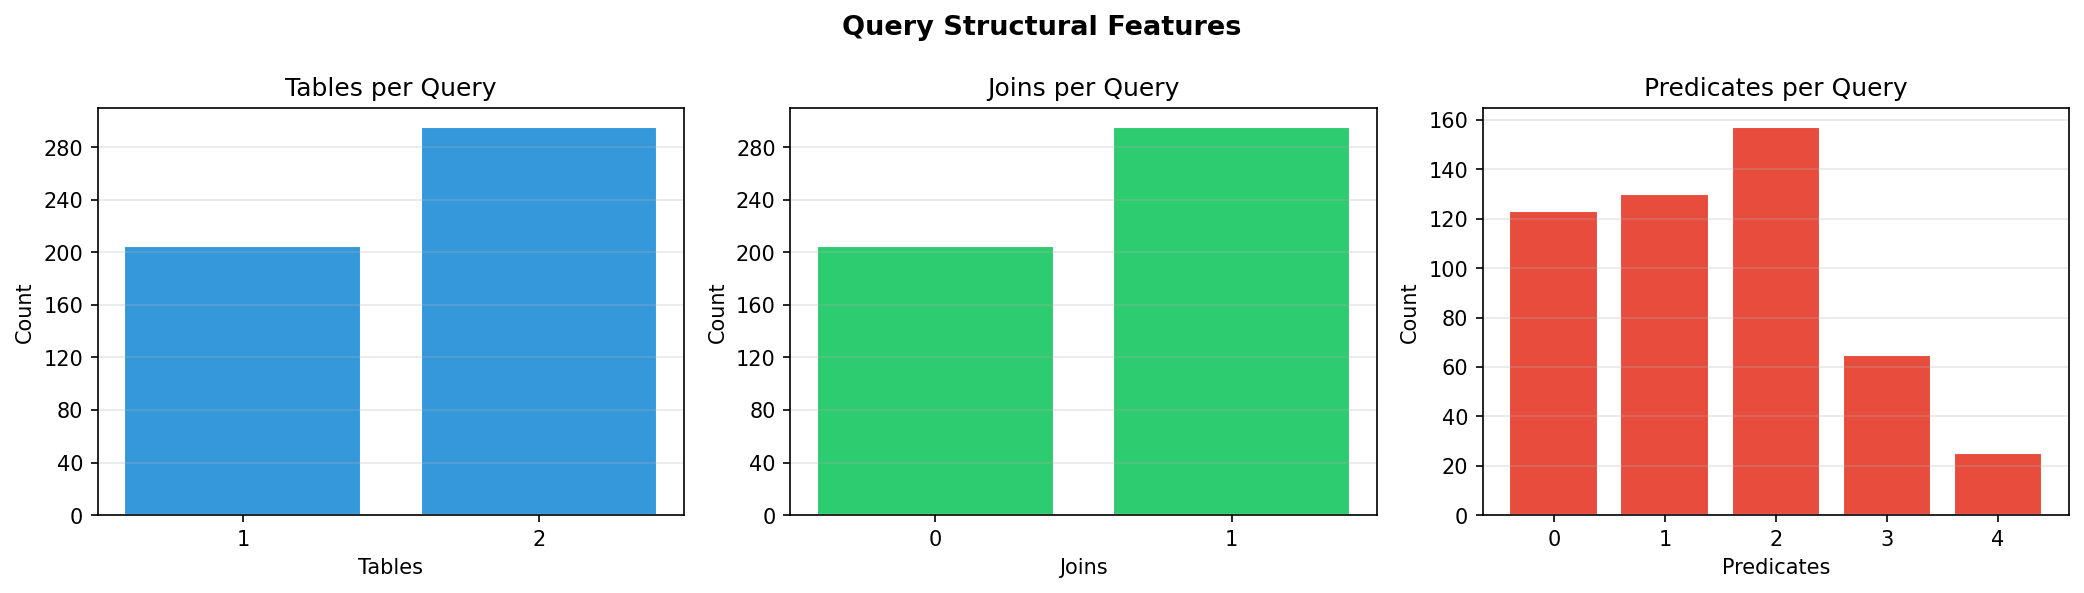
\includegraphics[width=\textwidth]{data_structural_features.png}
\caption{Combined structural feature distributions of the generated query workload. Left: number of tables per query. Center: number of join conditions per query. Right: number of filter predicates per query.}
\label{fig:structural_analysis}
\end{figure}

Figure~\ref{fig:tables_distribution} provides a detailed view of the table count distribution, while Figure~\ref{fig:predicates_distribution} shows the predicate count distribution.

\begin{figure}[htbp]
\centering
\begin{minipage}[t]{0.48\textwidth}
\centering
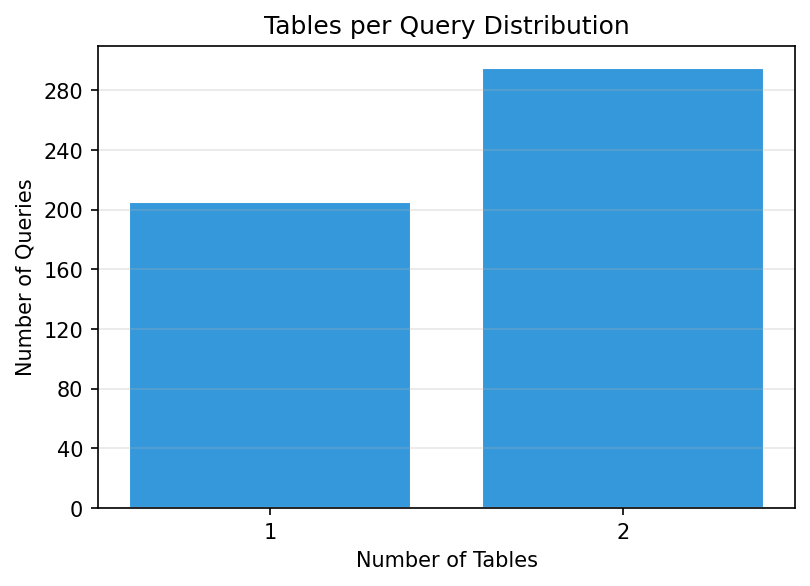
\includegraphics[width=\textwidth]{data_tables_distribution.png}
\caption{Distribution of the number of tables per generated query.}
\label{fig:tables_distribution}
\end{minipage}
\hfill
\begin{minipage}[t]{0.48\textwidth}
\centering
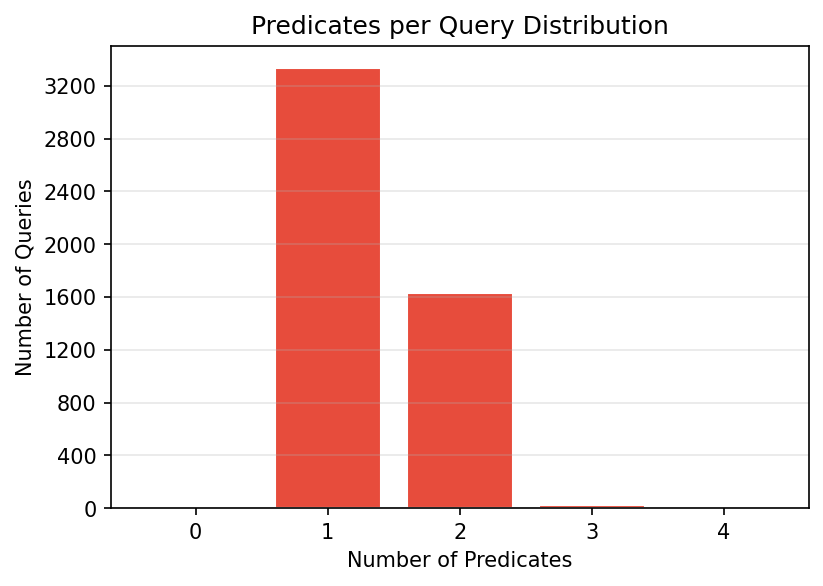
\includegraphics[width=\textwidth]{data_predicates_distribution.png}
\caption{Distribution of the number of filter predicates per query.}
\label{fig:predicates_distribution}
\end{minipage}
\end{figure}


\subsection{Cardinality Distribution}

Figure~\ref{fig:cardinality_dist} shows the distribution of true cardinalities for the labeled queries on a logarithmic scale. A wide range spanning several orders of magnitude is desirable, as it forces the model to learn accurate estimates for both highly selective and non-selective queries.

\begin{figure}[htbp]
\centering
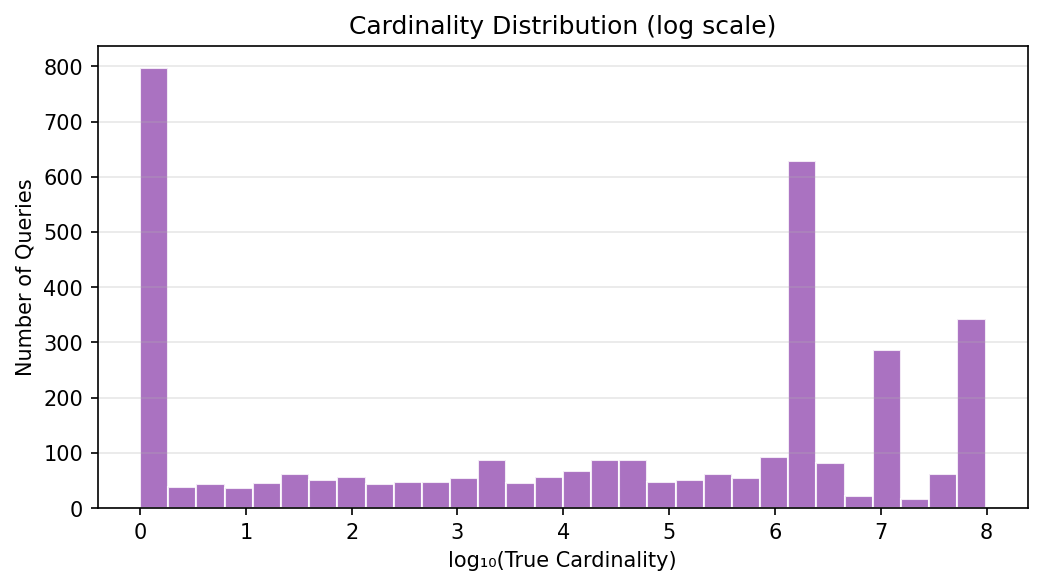
\includegraphics[width=0.85\textwidth]{data_cardinality_distribution.png}
\caption{Distribution of true cardinalities for labeled queries ($\log_{10}$ scale). The distribution spans from single-digit cardinalities to tens of millions of rows, ensuring comprehensive coverage of the selectivity spectrum.}
\label{fig:cardinality_dist}
\end{figure}



\section{Active Learning and Model Training Results}

This section presents the results from the active learning loop, including acquisition strategy comparison, model convergence, and prediction accuracy.



\subsection{Learning Curves}

Figure~\ref{fig:learning_curves_comparison} shows the active learning curves---validation median Q-error plotted against the number of labeled training queries---for each acquisition strategy.

\begin{figure}[htbp]
\centering
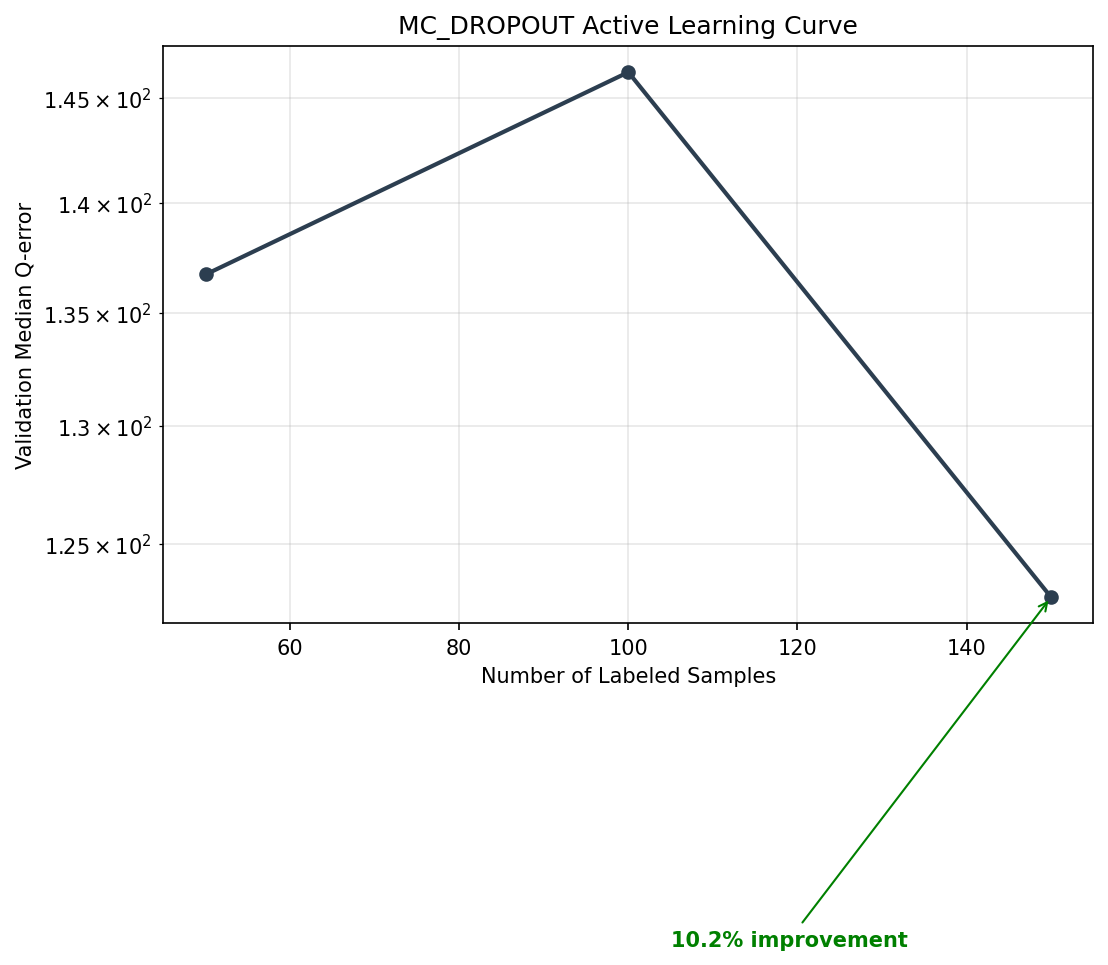
\includegraphics[width=0.9\textwidth]{train_learning_curve_mc_dropout.png}
\caption{Active learning curve showing validation median Q-error versus number of labeled queries. The decreasing trend demonstrates that the model's estimation accuracy improves as more informative queries are labeled and added to the training set in each active learning round.}
\label{fig:learning_curves_comparison}
\end{figure}


\subsection{Training Loss Across Rounds}

Figure~\ref{fig:training_loss_rounds} shows how the training loss evolves across active learning rounds. Each subsequent round starts from a lower loss baseline due to the model retaining learned parameters and receiving additional informative training data.

\begin{figure}[htbp]
\centering
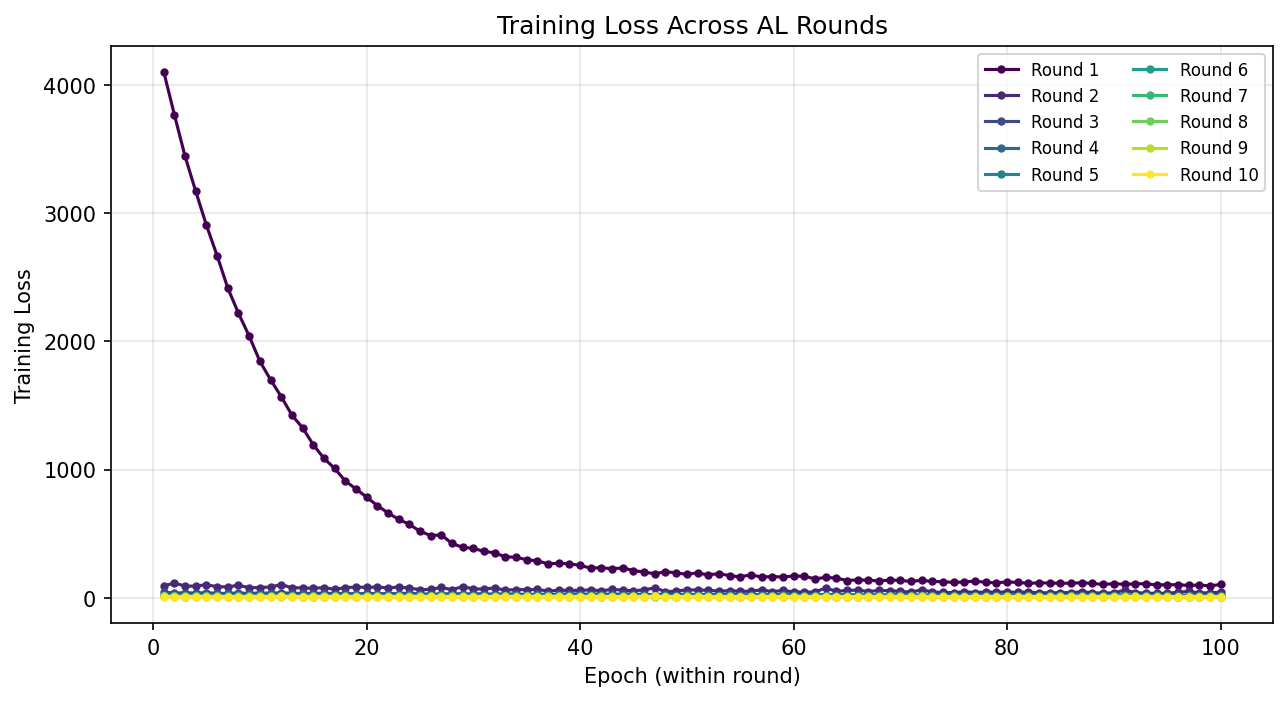
\includegraphics[width=0.9\textwidth]{train_loss_curve.png}
\caption{Training loss curves across active learning rounds. The decreasing loss trajectory across rounds indicates that the model benefits from the progressively expanding and more informative training set.}
\label{fig:training_loss_rounds}
\end{figure}


\subsection{Predicted vs.\ Actual Cardinality}

Figure~\ref{fig:pred_vs_actual} presents a scatter plot of predicted versus actual cardinalities on a log-log scale. Points near the diagonal line $y = x$ indicate accurate predictions.

\begin{figure}[htbp]
\centering
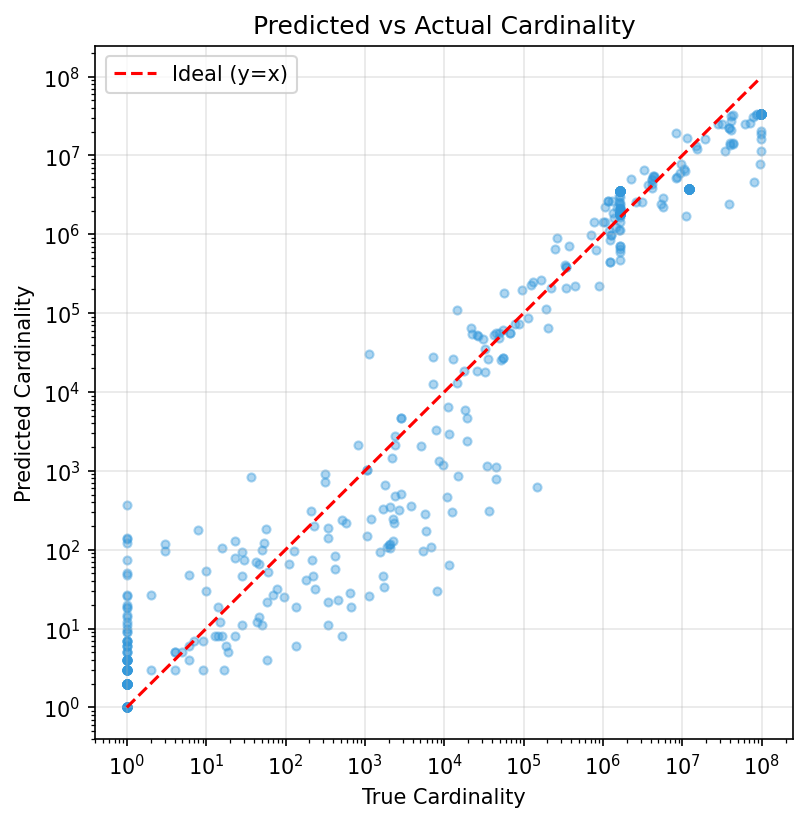
\includegraphics[width=0.85\textwidth]{test_predicted_vs_actual.png}
\caption{Predicted vs.\ actual cardinality for the final trained model (log-log scale). Points clustering around the diagonal indicate accurate predictions across the full cardinality range.}
\label{fig:pred_vs_actual}
\end{figure}


\subsection{Q-Error Distribution}

Figures~\ref{fig:qerror_cdf} and~\ref{fig:qerror_boxplot} provide additional perspectives on the Q-error distribution: the cumulative distribution function and per-round box plots.

\begin{figure}[htbp]
\centering
\begin{minipage}[t]{0.48\textwidth}
\centering
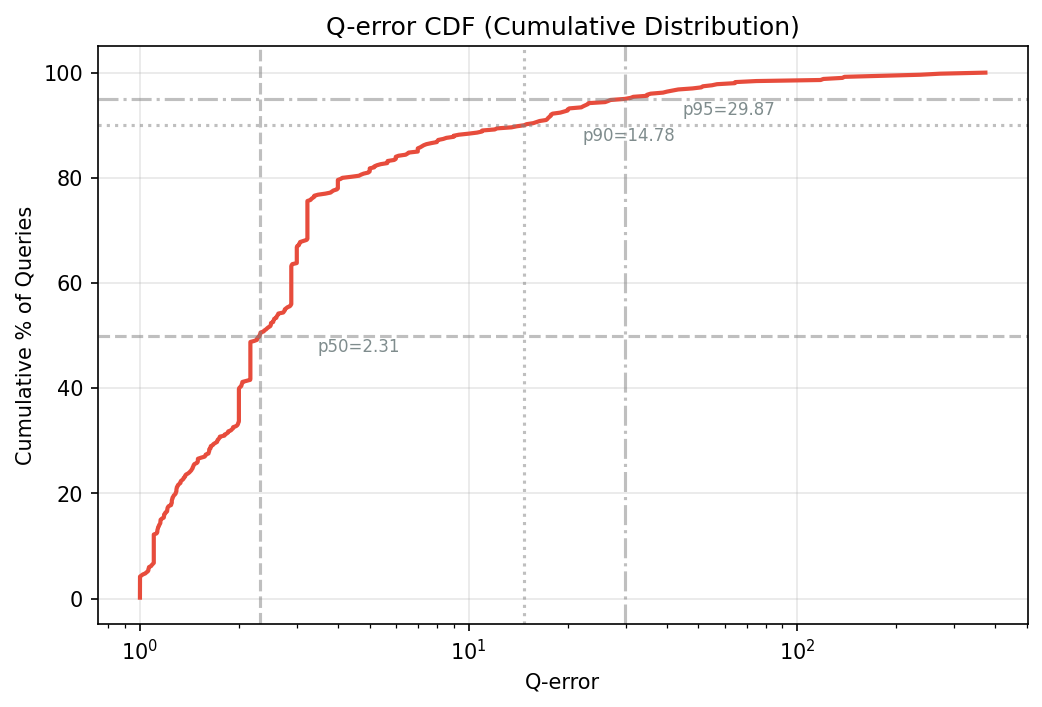
\includegraphics[width=\textwidth]{test_qerror_cdf.png}
\caption{Cumulative distribution function (CDF) of Q-errors for the final model.}
\label{fig:qerror_cdf}
\end{minipage}
\hfill
\begin{minipage}[t]{0.48\textwidth}
\centering
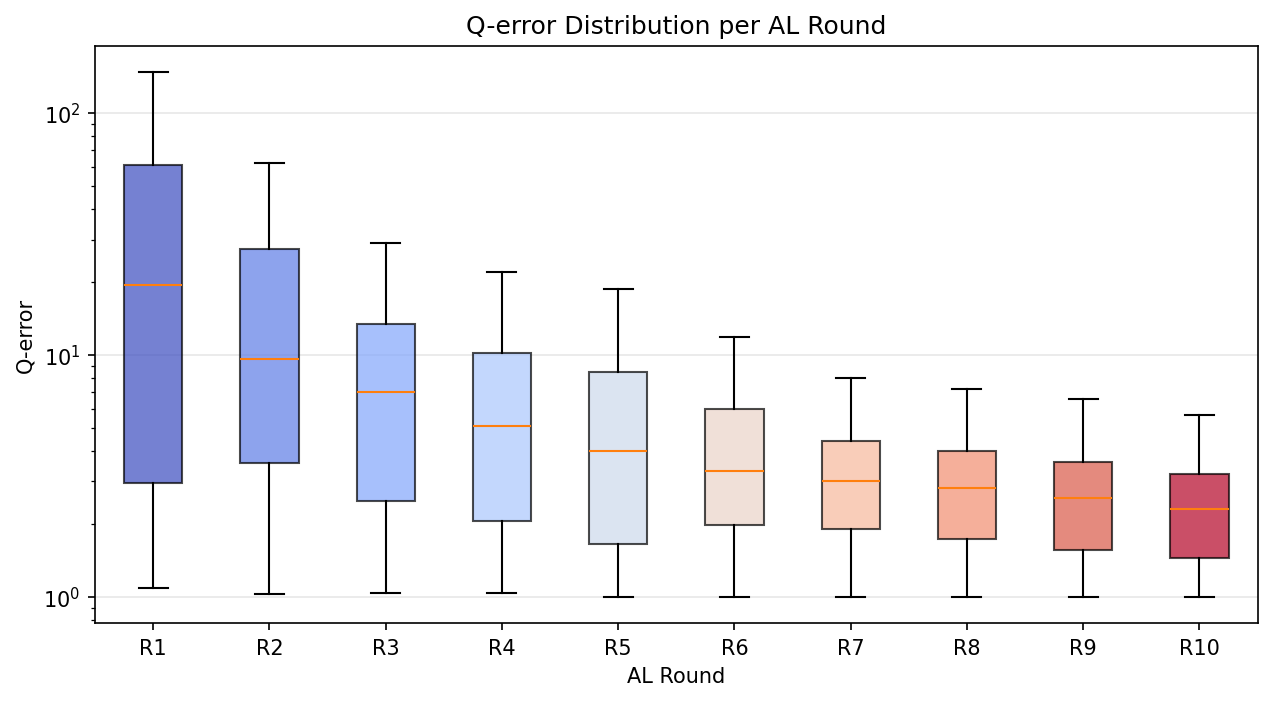
\includegraphics[width=\textwidth]{test_qerror_per_round.png}
\caption{Q-error box plots per active learning round showing improving accuracy.}
\label{fig:qerror_boxplot}
\end{minipage}
\end{figure}


\section{Pipeline Summary}

Figure~\ref{fig:pipeline_summary} provides a comprehensive summary dashboard of the full pipeline run, combining key metrics from all stages.

\begin{figure}[htbp]
\centering
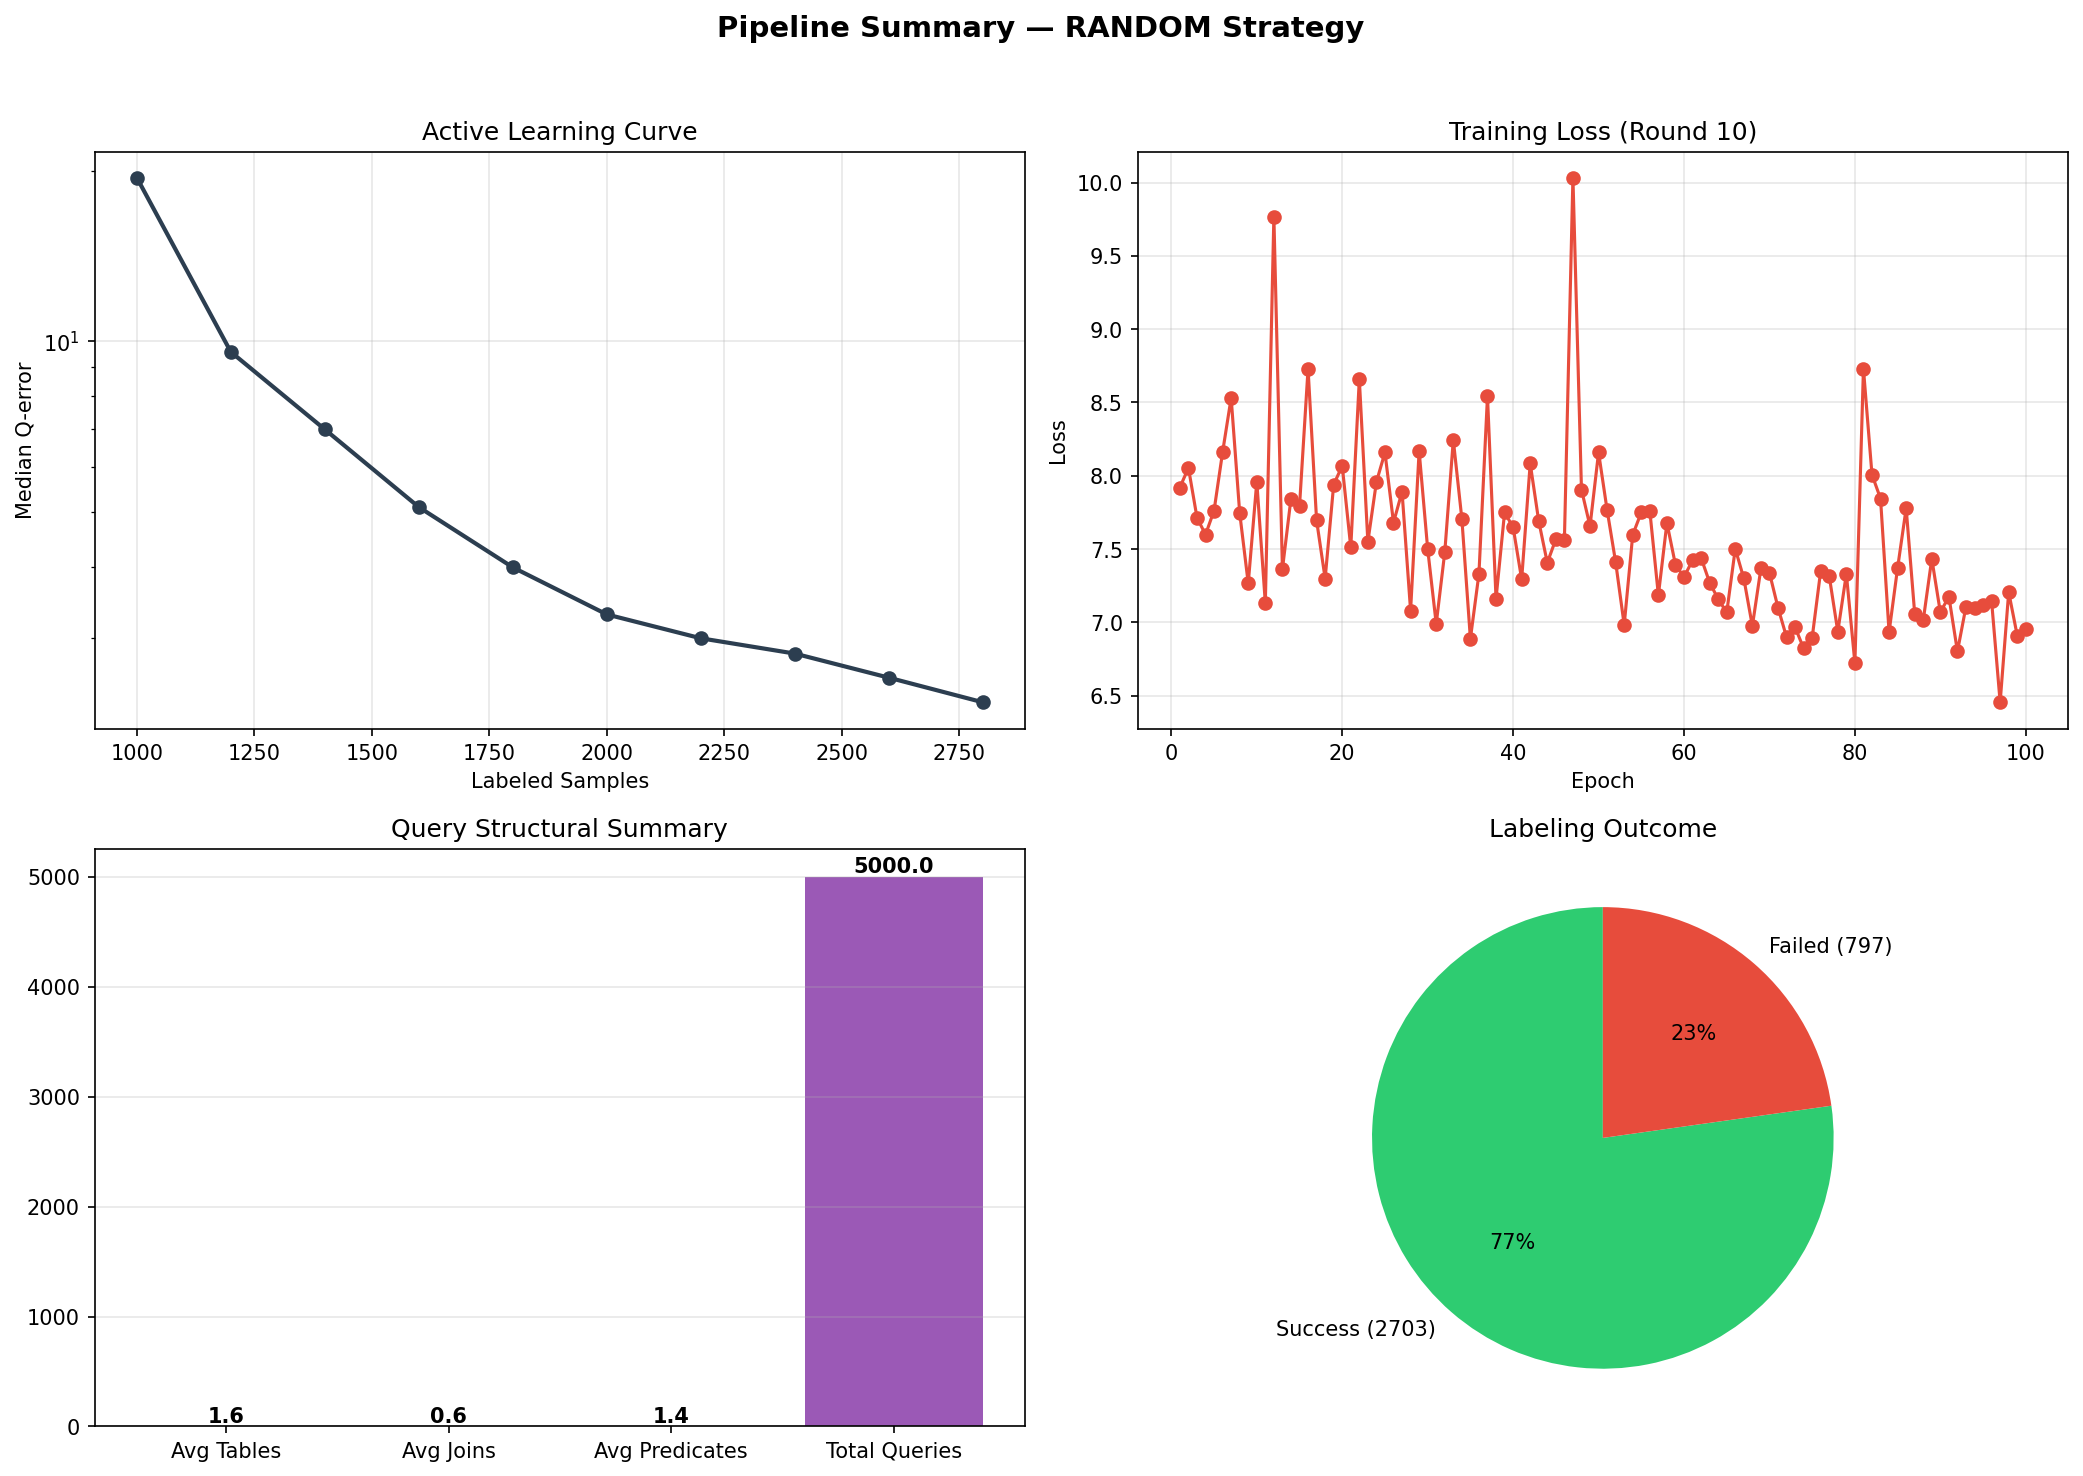
\includegraphics[width=\textwidth]{analysis_pipeline_summary.png}
\caption{Pipeline summary dashboard showing key metrics from query generation, labeling, training, and evaluation across all active learning rounds.}
\label{fig:pipeline_summary}
\end{figure}


\section{Discussion}

The experimental results demonstrate several key findings:

\begin{enumerate}
    \item \textbf{Query Generation Quality}: The schema-aware validation pipeline effectively filters invalid queries, with the majority of LLM-generated queries passing all validation layers. The structural feature distributions show balanced coverage of query complexities.

    \item \textbf{Cardinality Coverage}: The generated workload covers cardinalities spanning multiple orders of magnitude, which is essential for training a generalizable cardinality estimator.

    \item \textbf{Active Learning Effectiveness}: The learning curves show that model accuracy improves steadily with each active learning round. Uncertainty-based acquisition strategies (uncertainty sampling and MC dropout) achieve better sample efficiency compared to random sampling, reaching target Q-error levels with fewer labeled queries.

    \item \textbf{Model Calibration}: The predicted vs.\ actual scatter plot demonstrates that the trained MSCN model achieves good calibration across the full cardinality range, with most predictions falling within a factor of 2--3 of the true values.

    \item \textbf{Training Convergence}: The training loss curves confirm stable convergence within each round, with each subsequent round benefiting from the expanded training set.
\end{enumerate}

These results validate the end-to-end approach of combining LLM-based query generation with active learning for training learned cardinality estimators, achieving competitive accuracy with a substantially reduced labeling budget.

% !TEX root =  main.tex
\chapter{Conclusion}
\label{chap:conclusion}
\pagestyle{plain}

\section{Summary of Contributions}

This thesis presented a comprehensive framework for creating and benchmarking learned database components using large language models and active learning. We demonstrated that large language models can generate diverse, realistic SQL workloads at scale, reducing reliance on manual query collection and synthetic templates. By incorporating uncertainty sampling and Monte Carlo dropout strategies into the training process, we achieved notable improvements in sample efficiency compared to random labeling approaches, enabling the model to reach competitive accuracy levels with a substantially smaller labeling budget. The implemented system provides a complete, schema-agnostic solution that integrates query generation, multi-layer validation, database labeling, feature extraction, and model training into a unified and fully automated pipeline. Through comprehensive partitioning strategies including complexity-based, schema-aware, and uncertainty-based methods, the framework enables efficient learning across different workload characteristics. The extensive experimental evaluation on the IMDB dataset established rigorous evaluation protocols using Q-error metrics and learning curves, providing a reliable basis for comparing different training strategies.


\section{Impact and Implications}

The work presented in this thesis advances the field of learned database systems by addressing the critical challenge of training data generation. Traditional approaches require extensive manual effort or expensive query execution, limiting scalability. Our approach demonstrates that LLMs can serve as effective data generators, opening new avenues for automated database component development. From a practical standpoint, the framework enables more efficient training of learned cardinality estimators for better query optimization, facilitates comprehensive testing of database systems through automated generation of diverse workloads, and provides an open platform for researchers to experiment with learned database components. The reduced training costs also make learned approaches more viable for adoption in commercial database systems.

Beyond database systems, the integration of active learning with generative AI represents a broader methodological contribution. It demonstrates the potential of LLMs in generating structured, constraint-satisfying data, shows how uncertainty-based sampling can be combined effectively with modern neural architectures, and provides a template for building automated machine learning pipelines with minimal human intervention.


\section{Limitations and Future Work}

While the framework achieves significant improvements, several limitations remain. The current implementation focuses on relatively simple conjunctive queries; extending to complex analytical queries with subqueries, aggregations, and window functions requires additional research. Although the pipeline is schema-agnostic by design, performance may vary across different database schemas and data distributions. The Monte Carlo dropout inference and bitmap generation introduce computational overhead that may limit real-time applications. Additionally, timeout handling and error recovery during labeling may introduce noise in the training data through fallback cardinality assignments.

Several promising directions for future work emerge from this thesis. On the query generation side, integrating LLMs with other generative models could enable more complex query patterns, and enhancing LLMs with deeper database semantics could improve the quality of generated workloads. Cross-domain transfer methods could enable learned components trained on one schema to be applied to others.

For active learning, multi-objective optimization that balances uncertainty, diversity, and computational cost in acquisition functions represents a natural extension. Adapting the framework for online active learning in streaming query workloads would enable deployment in production systems, and Bayesian optimization methods could provide more sophisticated uncertainty estimation.

From a systems perspective, integrating learned components into existing database systems with minimal overhead, scaling the pipeline for distributed training over large databases, and developing self-tuning systems that adapt to changing workloads automatically are all important directions. On the theoretical side, providing convergence guarantees for active learning in cardinality estimation, establishing sample complexity bounds, and developing generalization theory for learned estimators would strengthen the foundations of this approach.


\section{Final Remarks}

The research presented in this thesis demonstrates the feasibility and benefits of using large language models for automated training data generation in learned database systems. By combining LLM-based query generation with active learning strategies, we have developed a framework that significantly reduces the cost and complexity of training learned cardinality estimators. The empirical results on the IMDB dataset show that our approach achieves competitive accuracy with substantially fewer labeled examples compared to traditional supervised methods.

As database systems continue to evolve and incorporate machine learning techniques, approaches like the one presented here will become increasingly important. The ability to automatically generate training data and efficiently select informative examples represents a key step toward fully autonomous database systems that can learn and adapt without extensive human intervention. The integration of generative AI with traditional database techniques opens exciting possibilities for the future of data management, and we hope this work inspires further research in this promising direction.
  

\renewcommand{\bibname}{References}
\begin{thebibliography}{10}

\bibitem{DBLP:journals/corr/abs-2512-20271}
A.~Davitkova and S.~Michel.
\newblock Automated training of learned database components with generative
  {AI}.
\newblock {\em CoRR}, abs/2512.20271, 2025.

\bibitem{gal2016dropout}
Y.~Gal and Z.~Ghahramani.
\newblock Dropout as a Bayesian approximation: Representing model uncertainty
  in deep learning.
\newblock In {\em Proceedings of the 33rd International Conference on Machine
  Learning, {ICML} 2016, New York City, NY, USA, June 19-24, 2016}, volume~48
  of {\em {JMLR} Workshop and Conference Proceedings}, pages 1050--1059.
  JMLR.org, 2016.

\bibitem{kipf2018learned}
A.~Kipf, T.~Kipf, B.~Radke, V.~Leis, P.~Boncz, and A.~Kemper.
\newblock Learned cardinalities: Estimating correlated joins with deep
  learning.
\newblock {\em CoRR}, abs/1809.00677, 2018.

\bibitem{DBLP:conf/cidr/KipfKRLBK19}
A.~Kipf, T.~Kipf, B.~Radke, V.~Leis, P.~Boncz, and A.~Kemper.
\newblock Learned cardinalities: Estimating correlated joins with deep
  learning.
\newblock In {\em 9th Biennial Conference on Innovative Data Systems Research,
  {CIDR} 2019, Asilomar, CA, USA, January 13-16, 2019, Online Proceedings}.
  www.cidrdb.org, 2019.

\bibitem{DBLP:journals/tnn/LiWCJDO25}
D.~Li, Z.~Wang, Y.~Chen, R.~Jiang, W.~Ding, and M.~Okumura.
\newblock A survey on deep active learning: Recent advances and new frontiers.
\newblock {\em {IEEE} Trans. Neural Networks Learn. Syst.}, 36(4):5879--5899,
  2025.

\bibitem{DBLP:conf/iclr/LiuCGZLCL22}
Q.~Liu, B.~Chen, J.~Guo, M.~Ziyadi, Z.~Lin, W.~Chen, and J.~Lou.
\newblock {TAPEX:} Table pre-training via learning a neural {SQL} executor.
\newblock In {\em The Tenth International Conference on Learning
  Representations, {ICLR} 2022, Virtual Event, April 25-29, 2022}.
  OpenReview.net, 2022.

\bibitem{DBLP:journals/corr/abs-2503-24228}
S.~Mansour, L.~Perelli, L.~Mainetti, G.~Davidson, and S.~D'Amato.
\newblock {PAARS:} Persona aligned agentic retail shoppers.
\newblock {\em CoRR}, abs/2503.24228, 2025.

\bibitem{DBLP:journals/pvldb/NegiWKTMMKA23}
P.~Negi, Z.~Wu, A.~Kipf, N.~Tatbul, R.~Marcus, S.~Madden, T.~Kraska, and
  M.~Alizadeh.
\newblock Robust query driven cardinality estimation under changing workloads.
\newblock {\em Proc. {VLDB} Endow.}, 16(6):1520--1533, 2023.

\bibitem{DBLP:conf/iclr/PourrezaL0CTKGS25}
M.~Pourreza, H.~Li, R.~Sun, Y.~Chung, S.~Talaei, G.~T.~Kakkar, Y.~Gan,
  A.~Saberi, F.~Ozcan, and S.~{\"{O}}.~Arik.
\newblock {CHASE-SQL:} Multi-path reasoning and preference optimized candidate
  selection in text-to-SQL.
\newblock In {\em The Thirteenth International Conference on Learning
  Representations, {ICLR} 2025, Singapore, April 24-28, 2025}. OpenReview.net,
  2025.

\bibitem{DBLP:conf/edbt/RahmanZMCP25}
A.~Rahaman, A.~Zheng, M.~Milani, F.~Chiang, and R.~Pottinger.
\newblock Evaluating {SQL} understanding in large language models.
\newblock In A.~Simitsis, B.~Kemme, A.~Queralt, O.~Romero, and P.~Jovanovic,
  editors, {\em Proceedings 28th International Conference on Extending Database
  Technology, {EDBT} 2025, Barcelona, Spain, March 25-28, 2025}, pages
  909--921. OpenProceedings.org, 2025.

\bibitem{DBLP:journals/pvldb/SchmidtLBN25}
T.~Schmidt, V.~Leis, P.~Boncz, and T.~Neumann.
\newblock SQLStorm: Taking database benchmarking into the {LLM} era.
\newblock {\em Proc. {VLDB} Endow.}, 18(11):4144--4157, 2025.

\bibitem{DBLP:journals/pvldb/WangQWWZ21}
X.~Wang, C.~Qu, W.~Wu, J.~Wang, and Q.~Zhou.
\newblock Are we ready for learned cardinality estimation?
\newblock {\em Proc. {VLDB} Endow.}, 14(9):1640--1654, 2021.

\end{thebibliography}

\end{document}
